%!TEX root = main.tex
\section{Results}
\subsection{With and without Olympic Games}
Choosing $\beta=2$, $\gamma=0.5$ and an average transfer probability of $0.005$ we can run a simulation with and without the Olympic Games occurring with the previously described characteristics. We assume that the infection breaks out on the first day of the games in Rio De Janeiro. We set the initial infected population to 1000. In the following we will look at the SIR curves of 6 major cities.

With the Olympics occurring we get the following curves:
\begin{figure}[H]
	\centering
	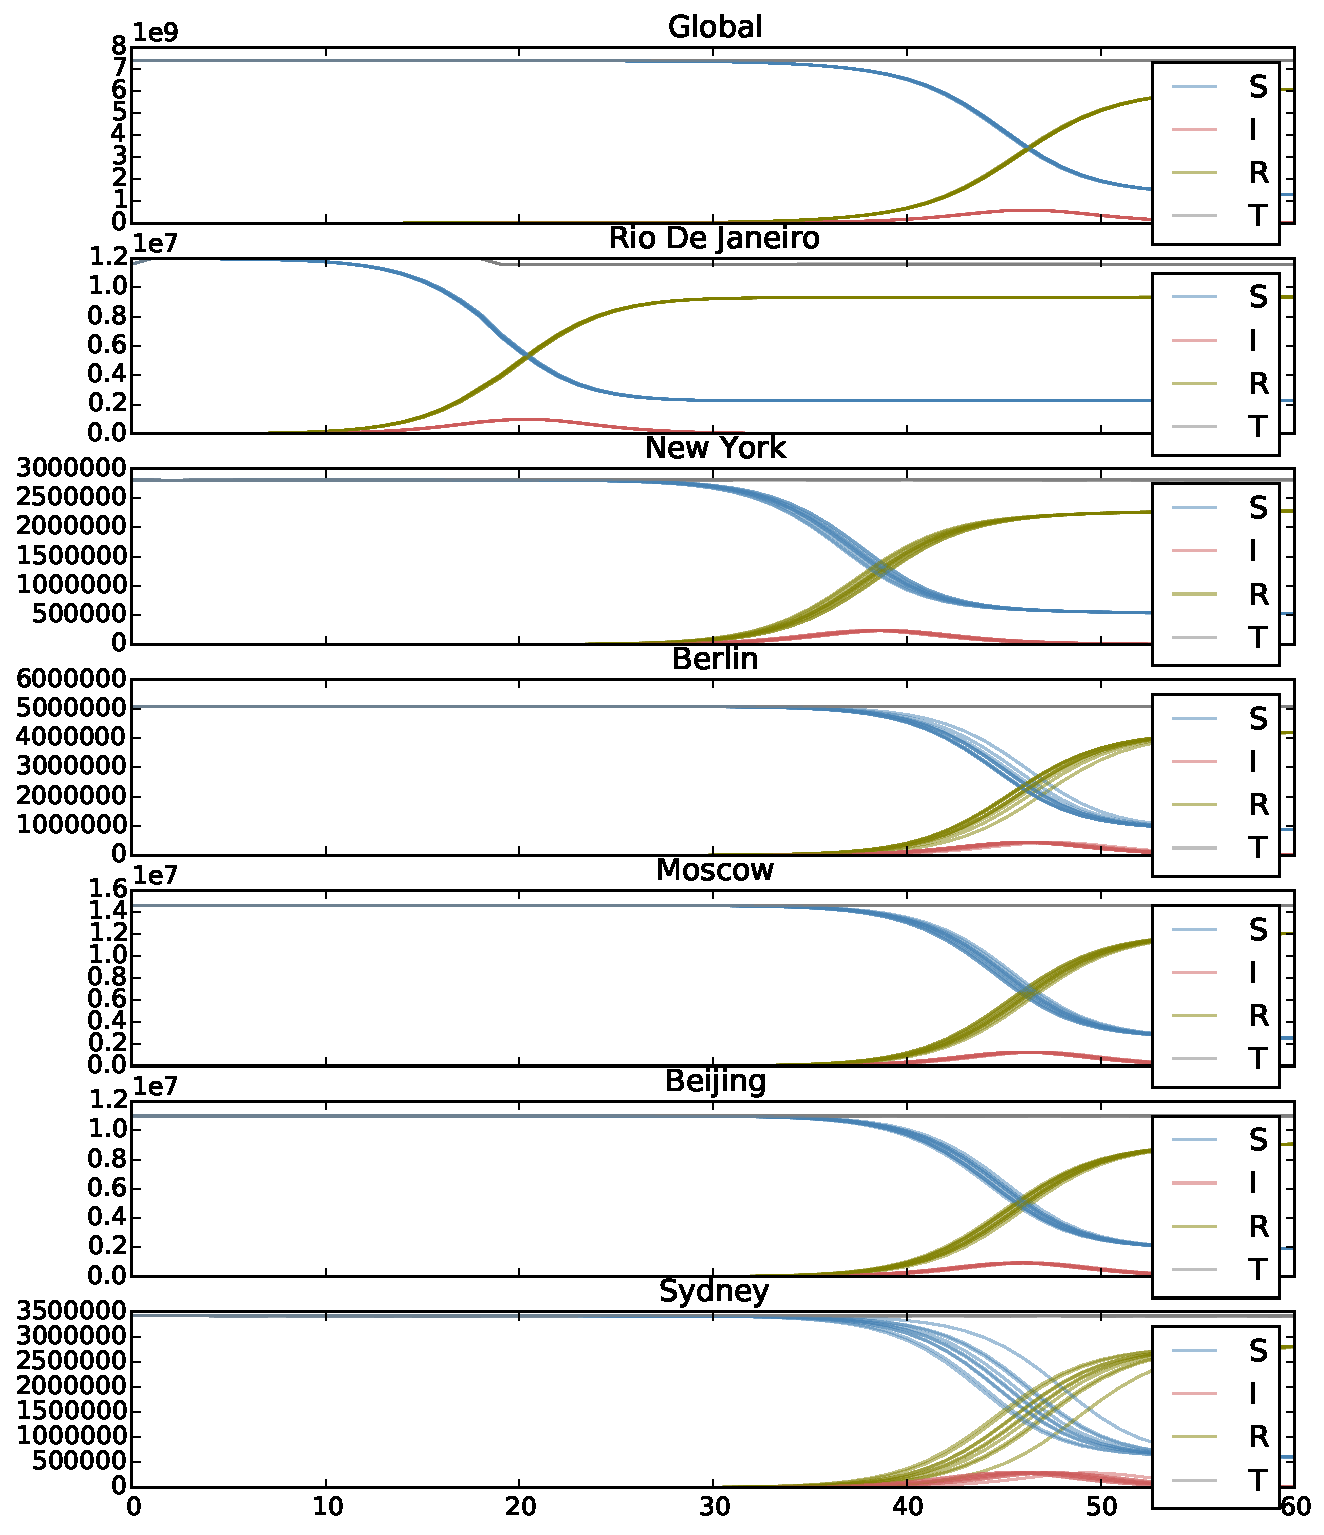
\includegraphics[width=1.0 \linewidth]{plots/rio-0-18-380000.pdf}
	\caption{10 simulations with Olympic Games. Time in days on the x-axis and number of people on the y-axis}
\end{figure}

From the above plot we see that except for New York which seems to be infected quickest, the other major cities all seem to reach peak infection rates at the same time. 

\begin{figure}[H]
	\centering
	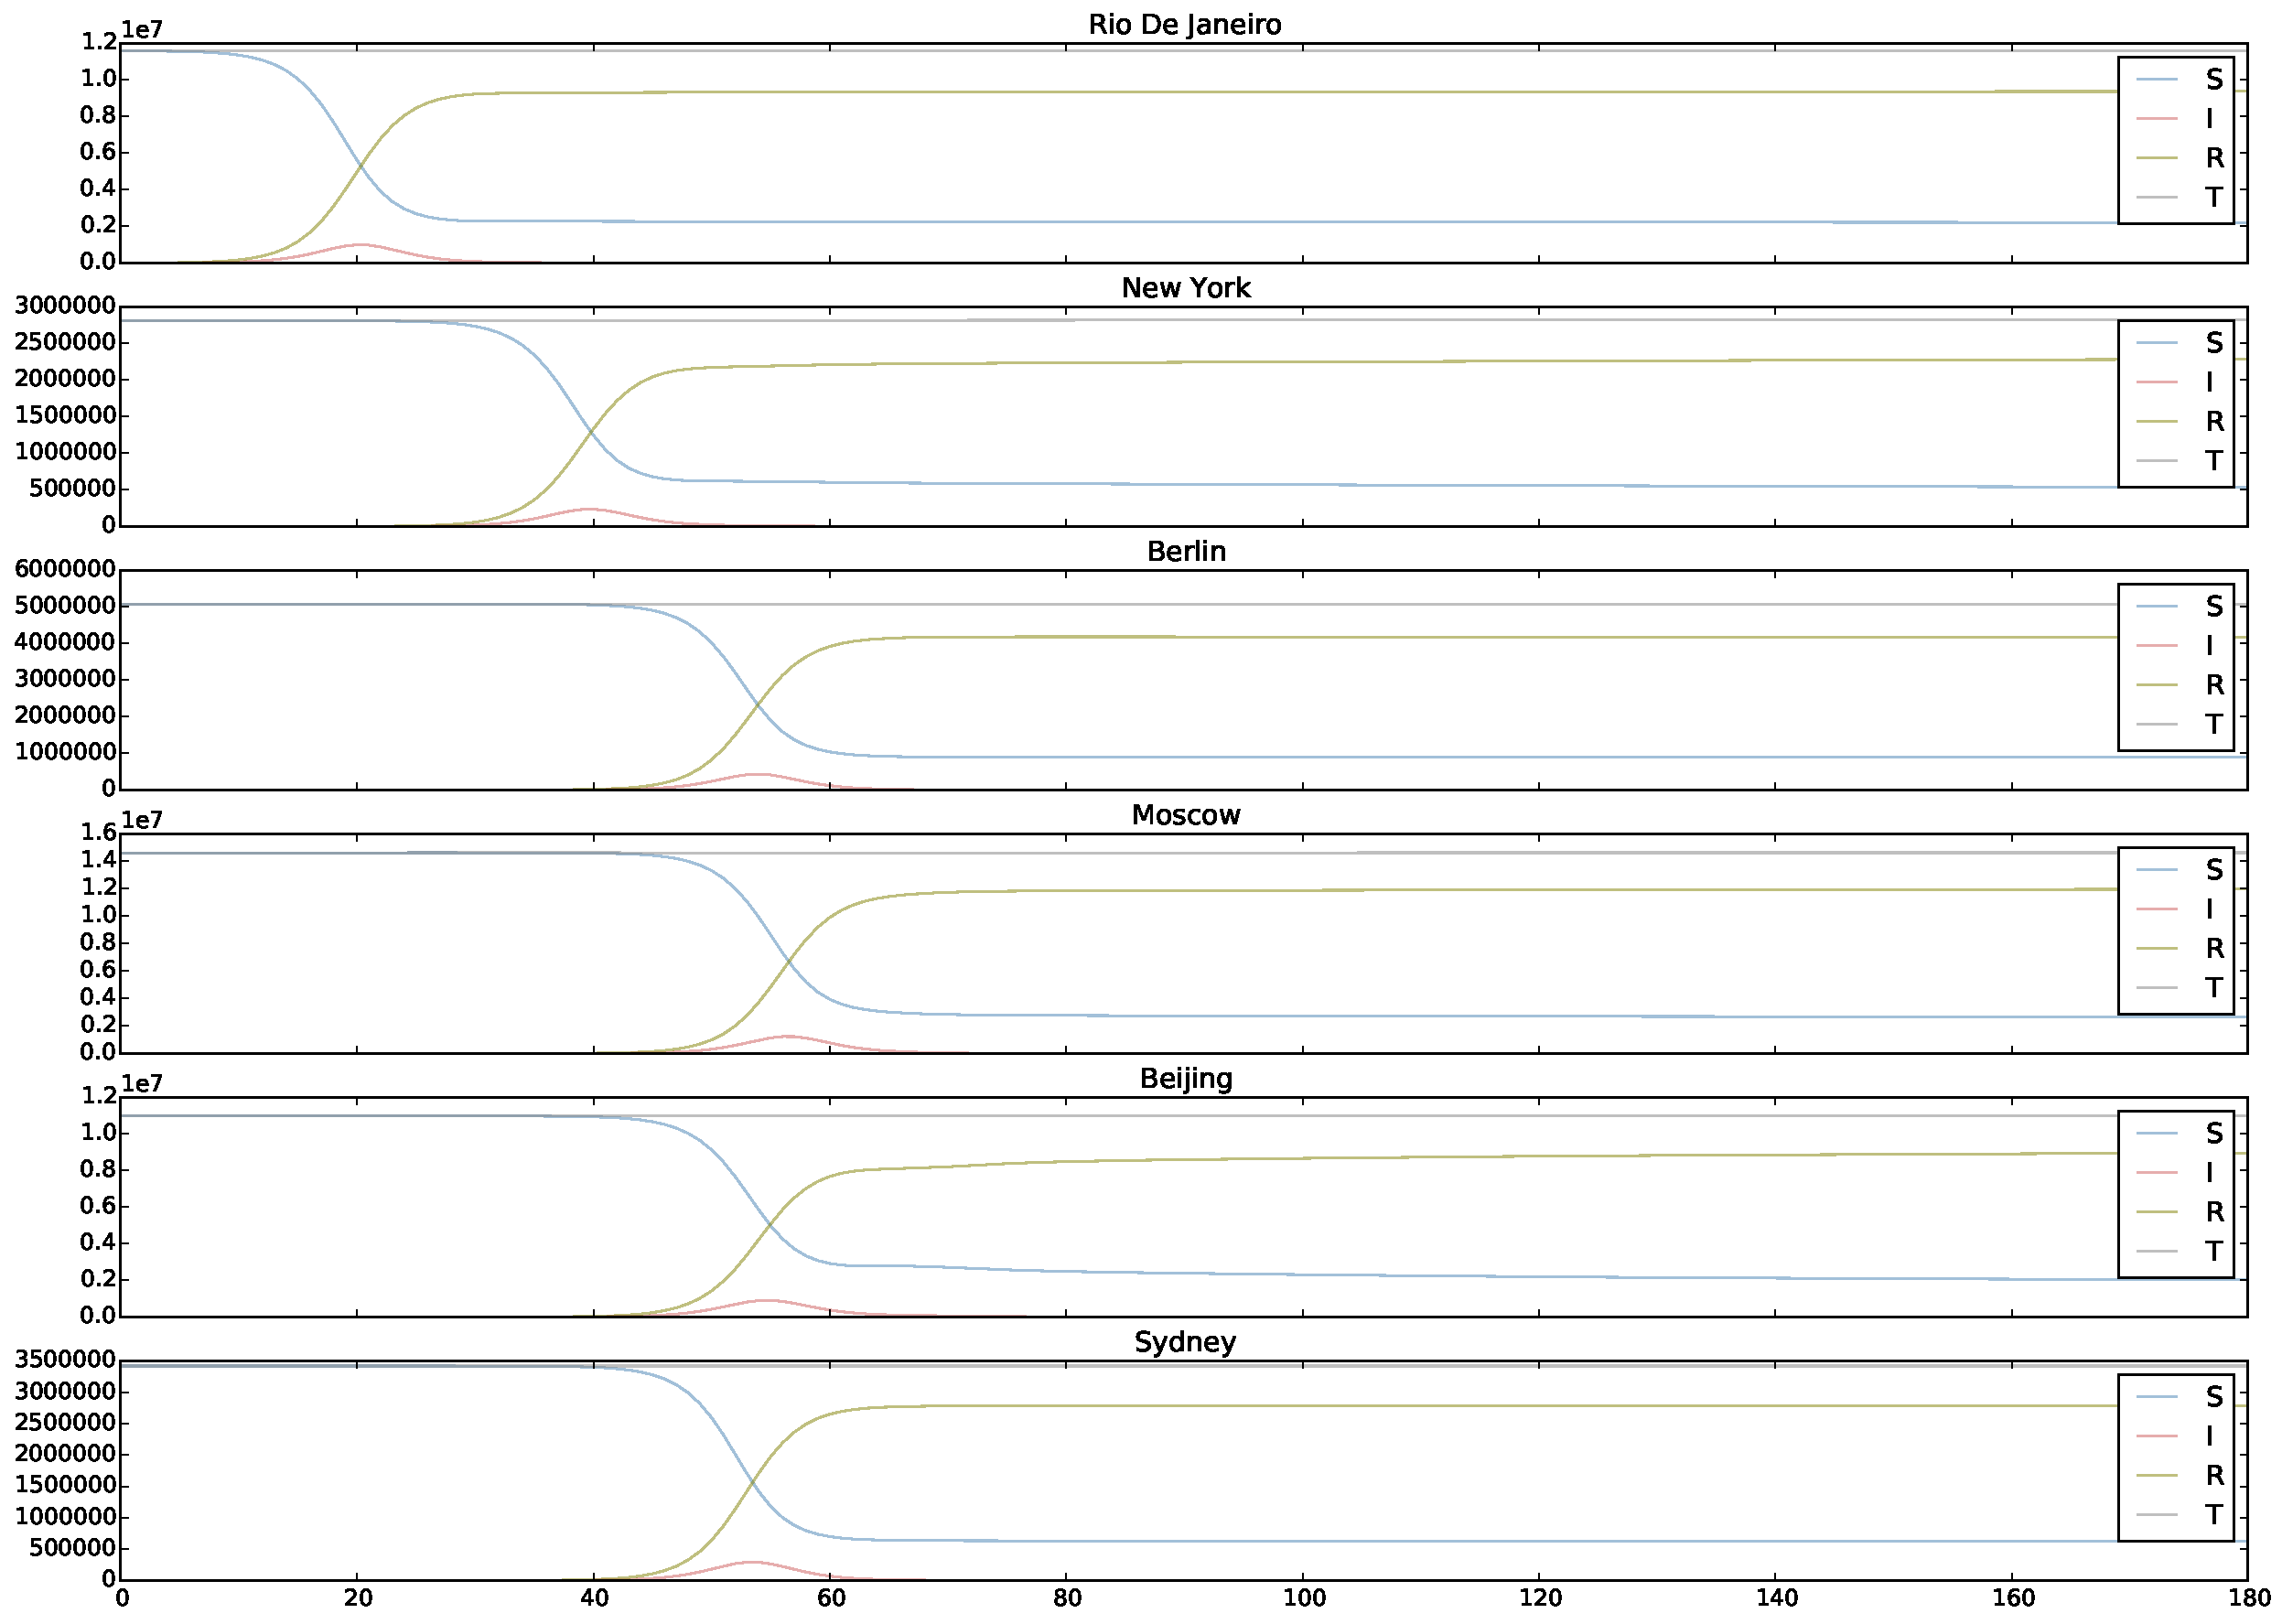
\includegraphics[width=1.0 \linewidth]{plots/no_rio.pdf}
	\caption{10 simulations without Olympic Games. Time in days on the x-axis and number of people on the y-axis}
\end{figure}

If one looks closely at the plot above we see that without the Olympic Games peak infections occur later for especially Moscow, Beijing and Sydney. The is perhaps a bit easier to see in the table below:

\begin{table}[H]
	\centering
	\begin{tabular}[H]{c | c | c}
Observation & With OL & Without OL \\ \hline 
 Peak amount Global [million]& $590.5\pm 0.94 (0.02)$ & $291.5 \pm 1.41 (0.01)$\\ 
 Peak time Global & $46.0\pm 0.00( 0.00)$ & $67.0 \pm 0.00 (0.00)$\\ 
 Peak time Rio & $20.2\pm 0.30( 0.26)$ & $20.0 \pm 0.00 (0.00)$\\ 
 Peak time New York & $38.6\pm 0.50( 0.52)$ & $38.3 \pm 0.59 (0.50)$\\ 
 Peak time Berlin & $46.4\pm 0.77( 0.56)$ & $53.7 \pm 0.35 (0.30)$\\ 
 Peak time Moscow & $46.1\pm 0.23( 0.23)$ & $56.3 \pm 0.35 (0.28)$\\ 
 Peak time Beijing & $46.0\pm 0.00( 0.00)$ & $55.0 \pm 0.34 (0.30)$\\ 
 Peak time Sydney & $46.3\pm 0.83( 0.73)$ & $53.3 \pm 0.48 (0.51)$
\end{tabular}
	\caption{Results of 10 simulations with and without Olympic Games. Table contains the peak times and amounts for the number of infected individuals.}
\end{table}]

\todo{comment on table}

\subsection{Visualization of result}
When studying a virus outbreak it is interesting to see exactly how the virus spreads. We have thus created an animation on a world map showing where each region is represented as a dot (scaled according to the population size) and the color of the dot represents the fraction infected. With this visualization the difference between including the Olympic Games and including becomes more apparent.

\begin{figure}[H]
	\centering
	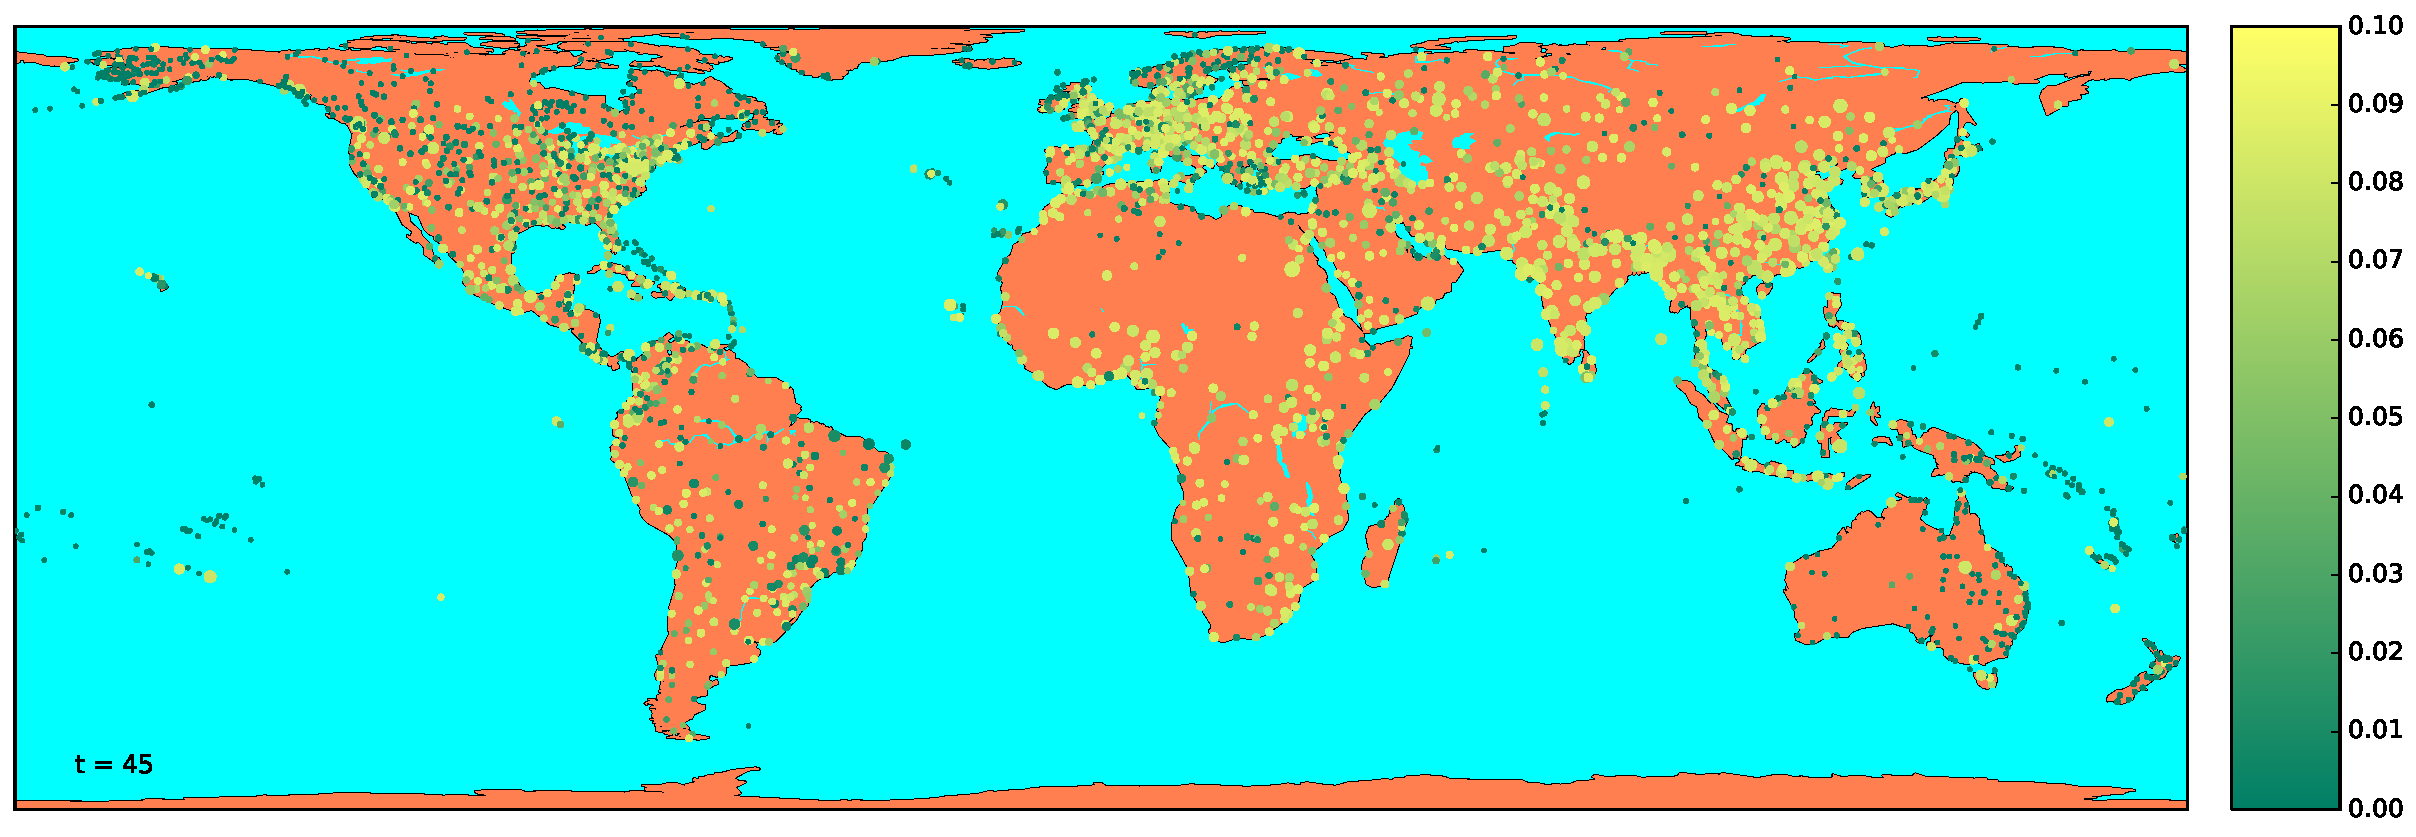
\includegraphics[width=1.0 \linewidth]{plots/gifs/frames/rio-45}
	\caption{Frame 45 of animation with Olympic Games. The full animation can be viewed as a gif at
		\url{https://github.com/FrederikWR/course-02443-stochastic-virus-outbreaks/tree/master/report/plots/gifs/rio.mpg4}}
\end{figure}

\begin{figure}[H]
	\centering
	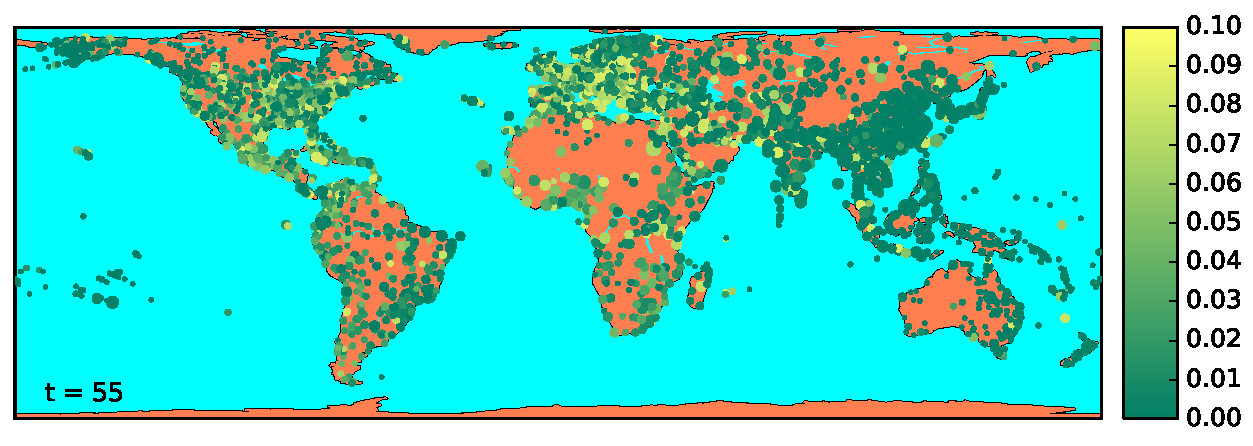
\includegraphics[width=1.0 \linewidth]{plots/gifs/frames/noRio-55}
	\caption{Frame 55 of animation without Olympic Games. The full animation can be viewed as a gif at
		\url{https://github.com/FrederikWR/course-02443-stochastic-virus-outbreaks/tree/master/report/plots/gifs/no\_rio.mpg4}}
\end{figure}


